\begin{figure}[h]
	\centering
	\missingfigure{Verteilungsdiagramm}		
	\caption{Verteilungsdiagramm}
	\label{fig:verteilungsdiagramm}
\end{figure}

\begin{tcolorbox}
	Das zukünftige Deployment des Systems wird mittels einem Verteilungsdiagramm modelliert.
	Weiterhin sollten wichtige oder eventuell undeutliche Zusammenhänge (z.B. warum Schnittstelle X genutzt wird) in einem Fließtext beschrieben werden.
\end{tcolorbox}

\begin{figure}[H]
	\centering
	\caption{Verteilungsdiagramm}
	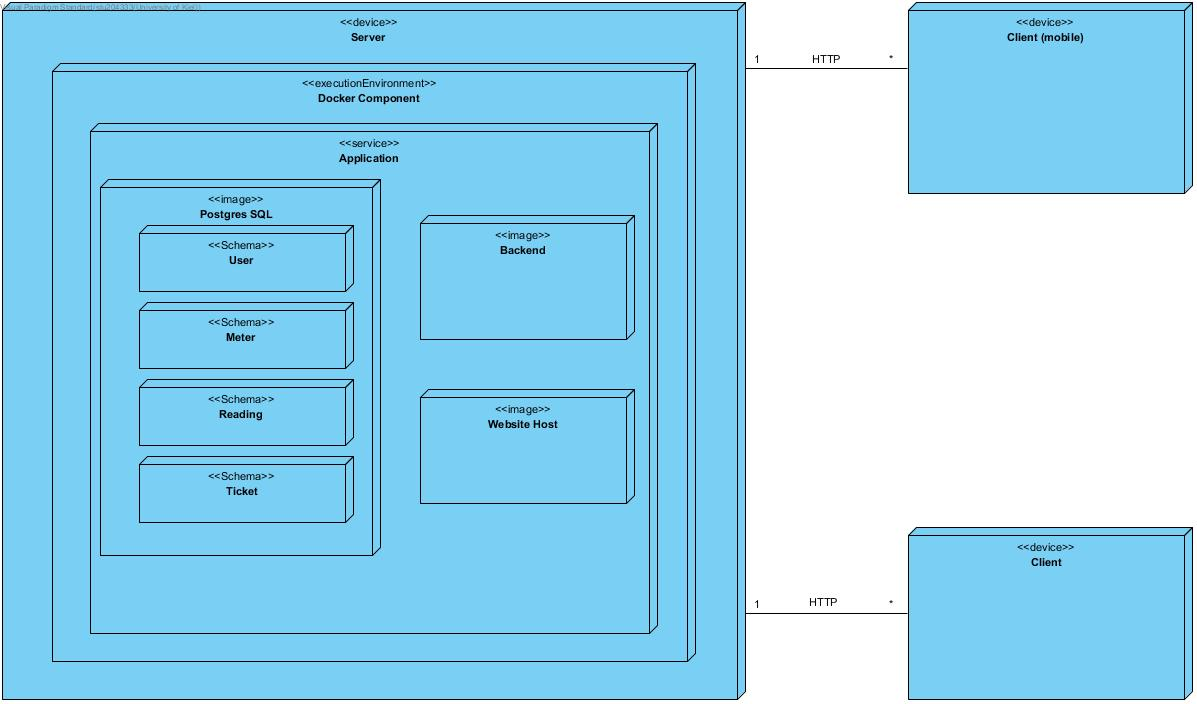
\includegraphics[width=16cm]{img/Diagrams/DeploymentDiagram}
\end{figure}
Im allgemeinen läuft die gesamte Software auf dem selben Server. Durch Docker werden die aufgabe aber in unterschiedlichen Containern benutzt werden.
So läuft in einem Container die Software für das Backend, die mittels einer REST-API mit dem Frontend kommuniziert. Clients können dann mittels HTTP anfragen an
das Backend stellen. Auch die App kommuniziert mittels HTTP mit dem Backend.
Ein Weiterer Container beinhaltet die SQL-Datenbank. Diese beinhaltet Schemata für Nutzer, Zähler, Zählerstände und Tickets.